\documentclass[a4paper,11pt]{article}
\usepackage{graphicx,listings,graphviz,a4wide}
%\usepackage[firstpage]{draftwatermark}
%\SetWatermarkLightness{0.5}
%\SetWatermarkScale{4}
\setcounter{tocdepth}{2}

\newcommand{\question}[2]{\medskip\par\noindent\textbf{#1}\\\hangindent=0.5cm#2}

\title{Report on OGO 2.2 \\ Software specification\\ Review formal specification group 3}
\author{
        Tim van Dalen, Tony Nan, Ferry Timmers, \\ Lasse Blaauwbroek, Femke Jansen, \\Jeroen Peters and Sander Breukink\\ OGO 2.2 group 6 \\
                Department of Computer Science\\
        Technical University Eindhoven\\
}
\date{\today}

\begin{document}

\maketitle

\begin{abstract}
ToDo: something about the purpose and structure of this document.
\end{abstract}

\newpage
	
	\tableofcontents
	\newpage
	
	\section{General remarks}
	%\lstset{
	tabsize=5,
	basicstyle=\small,
}

\begin{lstlisting}
Als een robot die meerdere hokjes in een keer kan afgleggen over een hint/
thuis/lopende band heen gaat, wat gebeurt er dan?
	Hint niets.
	Thuis wint.
	Lopende band gesleurd.
Als een hintvlak maar een hint kan geven, hoe kan hij dan een volgende 
keer een andere hint geven?
	Random.
Als een robot naar een vakje probeert te gaan wat bezet is, kan hij dan 
in dezelfde beurt nog een andere zet doen?
	Geen beurten, geen probleem.
Als een robot ergens op de lopende band terecht komt (niet begin / einde), 
wordt hij dan getransporteerd?
	Meegesleurd naar het einde.
Zijn de transportiebanden alleen een begin en eindvlakje? En als een robot 
nou aan het einde door robots is ingesloten, kan deze dan terug de lopende 
band op en verandert deze dan van richting?
	Aan het eind van een lopende band moet je je thuisvlak kunnen bereiken, 
	lopende banden zijn 1 kant op.
Hoe ver wordt een robot verplaatst als deze op een transportatieband 
(geen rotatie) terecht komt? 
	In 1x naar het einde.
Wat gebeurt er als het einde van de lopende band is ingesloten door 
defecte robots?
	-
Wat gebeurt er als er een defecte robot op een lopende band staat? 
Blijft deze staan of wordt hij getransporteerd?
	Je wisselt vakjes om, dus de lopende band stopt daar gewoon.
Kan een defecte robot ook een thuis/hintvlak blokkeren?
	Aantal soorten vakjes, die niet kunnen overlappen.
Kan een hintvlakje een of twee richtingen als hint geven?
	-
Kunnen transportatiebanden zowel rotatie als transport zijn?
	Beide, lopende band verdraaid random je rotatie.
Wat gebeurt er als een robot in het midden van een lopende band terecht komt, 
of zijn er alleen opstap en eindpunten?
	Gewoon naar het einde.
De twee robots hebben eigenlijk precies dezelfde functionaliteit aangezien er 
geen rondes zijn, en de robots dus zoveel moves in een tijdsunit mogen doen 
als ze willen. Daarom kan robot A net zo snel bewegen als robot B. En omdat 
robot B niet springt moet hij over alle vakjes heen en is het netto effect 
hetzelfde.
	Gewoon implementeren, het resultaat mag hetzelfde zijn. Het enige verschil 
	is dat robot B in zijn weg een hint tegen kan komen waar hij overheen 
	loopt. De robot krijgt deze hint dan niet te zien.

\end{lstlisting}

On Tuesday the 28th of Februari, we had a meeting with the stakeholders about the role of the controller. We assumed that the controller actually had to control something, but the stakeholder did not fully agree with us. In our MSCs the controller communicated with all other parts of the game (the players, the view and the board) and, for instance, first asked the board for two tiles that could be switched and then asked it to switch those. In the opninion of the stakeholder, the controller should merely serve as a communications tunnel and not make any decisions itself. Eventually, we reached a compromise. The controller still requests everything from the other parts, but all requests have been made automic, i.e. the tile request functions are now one function that the board handles by itself.

    ToDo
	
	\section{Remarks about the Z-specification}
	%\subsection{Use cases}
	\lstinputlisting{usecases/cases.txt}
\subsection{Use case diagram}
	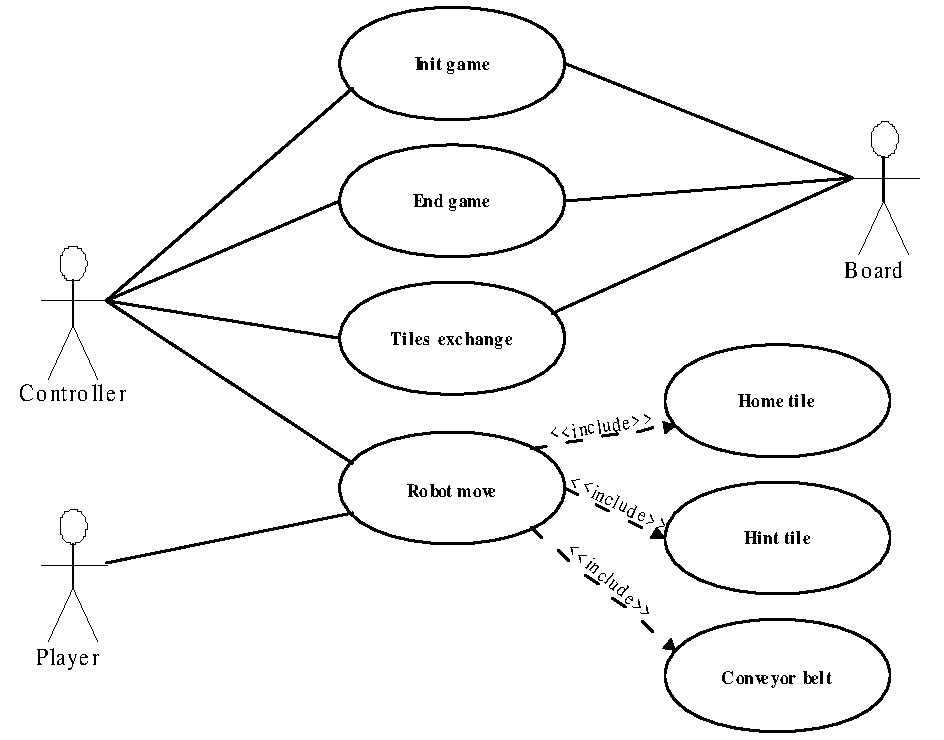
\includegraphics[width=\linewidth]{usecases/diagram.pdf}	

\subsection{High Level Message Sequence Chart}
	The following graph represents our high level message sequence chart and shows how a normal program flow is modeled by MSCs. The graph consists of two parts that run concurrently, the viewer part and the main game part. The viewer part will make sure the viewer updates regularly. The main game part follows the flow of a normal game. 
	
	\digraph[scale=0.4]{HMSC}{
begin2 [label="",shape="invtriangle"];
end2 [label="",shape="triangle"];
initview [label="Initialize viewer",shape="Mrecord"];
updateview [label="Update viewer",shape="Mrecord"];
begin2->initview;
initview->updateview;
updateview->updateview;
updateview->end2;
begin [label="",shape="invtriangle"];
end [label="",shape="triangle"];
p1 [label="",shape="point"];
p2 [label="",shape="point"];
p22 [label="",shape="point"];
p3 [label="",shape="point"];
p4 [label="",shape="point"];
p5 [label="",shape="point"];
p55 [label="",shape="point"];
p6 [label="",shape="point"];
p66 [label="",shape="point"];
p7 [label="",shape="point"];
p77 [label="",shape="point"];
p8 [label="",shape="point"];
init [label="Initialize",shape="Mrecord"];
mvreq [label="Robot move request",shape="Mrecord"];
mvrej [label="Reject move",shape="Mrecord"];
retnt [label="Return Normal tile",shape="Mrecord"];
retht [label="Return Hint tile",shape="Mrecord"];
retct [label="Return Conveyor tile",shape="Mrecord"];
retmt [label="Return Home tile",shape="Mrecord"];
ordex [label="Ordinary exchange",shape="Mrecord"];
spcex [label="Special exchange",shape="Mrecord"];
endgame [label="End game",shape="Mrecord"];
notrob1 [label="Notify robots",shape="Mrecord"];
notrob2 [label="Notify robots",shape="Mrecord"];
begin->p1;
p1->init;
init->p2;
p2->mvreq;
mvreq->p3;
p3->mvrej;
mvrej->p2;
p3->p4;
p4->retnt;
p4->retht;
p4->retct;
p4->retmt;
retnt->p5;
retht->p5;
retct->p5;
p5->p55;
p55->p66;
p66->p6;
p55->notrob1;
notrob1->p66;
p6->ordex;
p6->spcex;
ordex->p7;
spcex->p7;
p7->p77;
p77->p22;
p22->p2 [tailport=e];
p77->notrob2;
notrob2->p22;
retmt->endgame;
endgame->p8;
p8->p1;
p8->end;
}

	%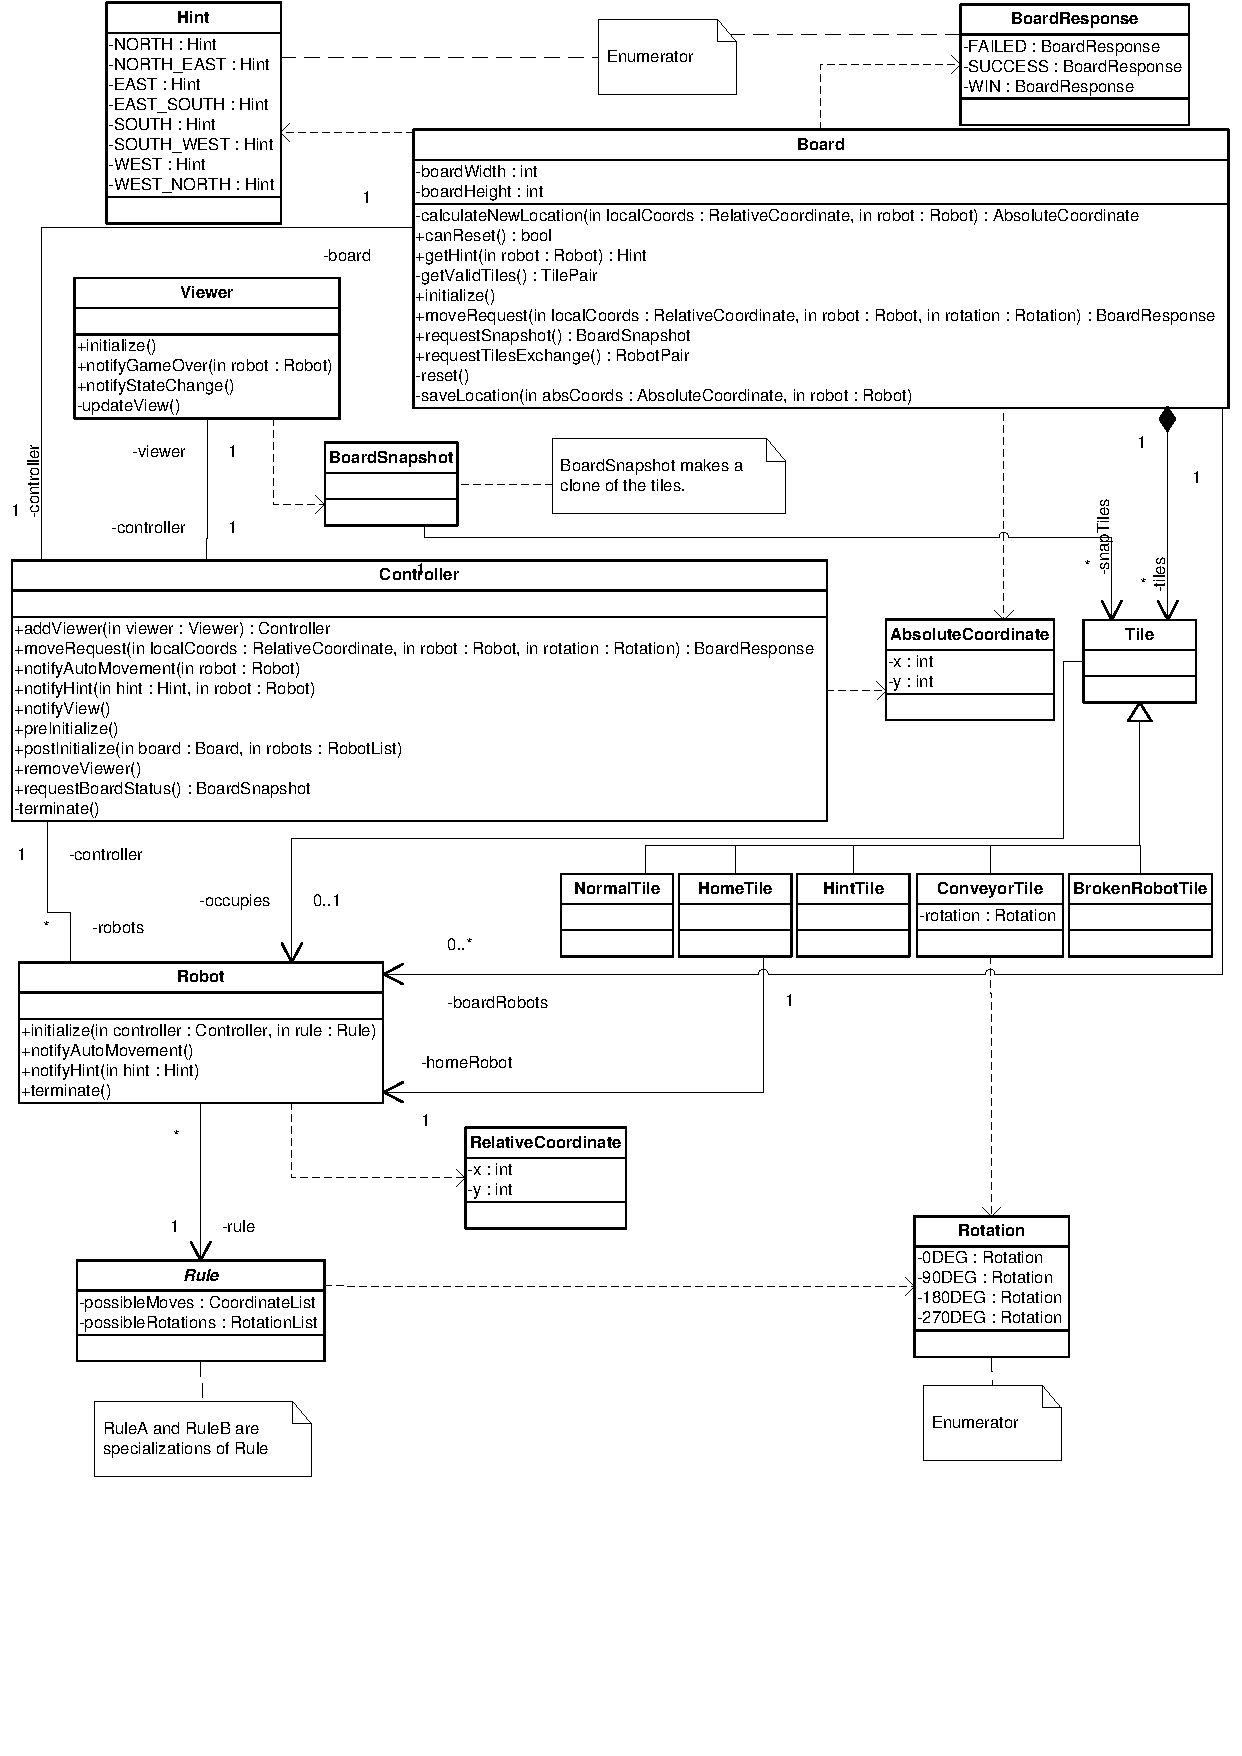
\includegraphics[width=\linewidth]{classdiagram}

\subsection{Message Sequence Charts}
	This section contains the message sequence charts for our use cases. Below every MSC is the location of the MSC in the High Level Message Sequence Chart.

	The world entity is not a real part of our MSCs, but rather a link to the outside world. When an internal action ends in '()' it's a function call to a private function of the entity. Otherwise, it's an action within the called function.

	Note: the symbol $\vdots$ denotes the start and end of a co-region.

	\subsubsection{Initialize viewer}
	The viewer is initialized by the world. Analogous to the HMSC, this happens concurrently to the Initialize MSC.
	
	\begin{msc}
msc
{

w [label="World"],
b [label="Board"],
c [label="Controller"],
v [label="Viewer"];

v box v [label=""],
b box b [label=""],
c box c [label=""],
w box w [label=""];

|||;

w => v [label="initialize(controller)"];
v rbox v [label="initialize"];
v => c [label="addViewer(viewer)"];
c >> v [label="self"];

... [label="board waits a predefined time"];

b rbox b [label="make snapshot"];
b -> c [label="notifyViewer(snapshot)"];
c -> v [label="notifyStateChange(snapshot)"];
v rbox v [label="updateView()"];

|||;

v box v [label="", textbgcolor="black"],
b box b [label="", textbgcolor="black"],
c box c [label="", textbgcolor="black"],
w box w [label="", textbgcolor="black"];

}
\end{msc}
\digraph[scale=0.5]{HMSC_init_view}{rankdir=LR;
p2 [label="",shape="point"];
init [label="Initialize",shape="Mrecord"];
initview [label="Initialize viewer",shape="Mrecord",style=filled];
mvreq [label="Robot move request",shape="Mrecord"];
init->initview;
initview->p2;
p2->mvreq
}


    	\subsubsection{Update viewer}
	During the game execution, the view will keep requesting the current board snapshot from the controller. This happens concurrently to the rest of the process. It can also request the board snapshot when it gets notified by the controller that the board has changed.
    	
	\begin{msc}
msc {

b [label="Board"],
c [label="Controller"],
d [label="Viewer"];

b box b [label=""],
d box d [label=""],
c box c [label=""];

|||;

d => c [label="requestBoardSnapshot()"];
c => b [label="requestBoardStatus()"];
b >> c [label="BoardSnapshot"];
c >> d [label="BoardSnapshot"];
d box d [label="updateView()"];

|||;

d box d [label="", textbgcolor="black"],
c box c [label="", textbgcolor="black"],
b box b [label="", textbgcolor="black"];

}
\end{msc}
\digraph[scale=0.5]{HMSC_upview}{
rankdir=LR;
end2 [label="",shape="triangle"];
initview [label="Initialize viewer",shape="Mrecord"];
updateview [label="Update viewer",shape="Mrecord",style=filled];
initview->updateview;
updateview->updateview;
updateview->end2;
} 

	\subsubsection{Initialize}
	When the game starts, the board is initialized. When this is done, the board sends a preInitialize to the controller. When the controller is done with that, the board will initialize all robots, which will reply with an 'OK' when done. When all robots have been initialized, the board sends a postInitialize to the controller. All entities are now initialized.
  	
	\begin{msc}
msc
{

a [label="Robot"],
b [label="Controller"],
c [label="Board"];

a box a [label=""],
b box b [label=""],
c box c [label=""];

|||;

b rbox b [label="initialize"];

b => a [label="initialize"];
a rbox a [label="initialize"];
a >> b [label=""];

b =>c [label="initialize(robotlist)"];
c rbox c [label="initliaze"];
c >>b [label="OK"];

|||;

a box a [label="", textbgcolor="black"],
b box b [label="", textbgcolor="black"],
c box c [label="", textbgcolor="black"];

}
\end{msc}
\digraph[scale=0.5]{HMSC_init}{rankdir=LR;
begin [label="",shape="invtriangle"];
p1 [label="",shape="point"];
p2 [label="",shape="point"];
init [label="Initialize",shape="Mrecord",style=filled];
mvreq [label="Robot move request",shape="Mrecord"];
begin->p1;
p1->init;
init->p2;
p2->mvreq
}

    	
	\subsubsection{Robot move request}
	A robot can make a move request with the controller, which will forward that to the board. The board will check the validity of the with the robots rule and then check the validity of the move at the current state of the board.

	\begin{msc}
msc
{

d [label="Board"],
c [label="Controller"],
a [label="Robot"],
r [label="Rule"];

d box d [label=""],
c box c [label=""],
a box a [label=""],
r box r [label=""];

|||;

a => c [label="moveRequest(localCoords, robot, rotation)"];
c => d [label="moveRequest(localCoords, robot, rotation)"];
d rbox d [label="get possible moves"], r note r [label="references the robot's ruleset"];
d rbox d [label="get possible rotations"];
d rbox d [label="check if robot can be placed"];

|||;

a box a [label="", textbgcolor="black"],
c box c [label="", textbgcolor="black"],
d box d [label="", textbgcolor="black"],
r box r [label="", textbgcolor="black"];

}
\end{msc}
\digraph[scale=0.5]{HMSC_req}{
rankdir=LR;
p2 [label="",shape="point"];
p3 [label="",shape="point"];
p4 [label="",shape="point"];
init [label="Initialize",shape="Mrecord"];
mvreq [label="Robot move request",shape="Mrecord",style=filled];
mvrej [label="Reject move",shape="Mrecord"];
retnt [label="Return Normal tile",shape="Mrecord"];
retht [label="Return Hint tile",shape="Mrecord"];
retct [label="Return Conveyor tile",shape="Mrecord"];
retmt [label="Return Home tile",shape="Mrecord"];
init->p2;
p2->mvreq;
mvreq->p3;
p3->mvrej;
mvrej->p2;
p3->p4;
p4->retnt;
p4->retht;
p4->retct;
p4->retmt;
}


	\subsubsection{Return Normal tile}
	If the move request is okay, and the robot is moved to a normal tile, the board will return \emph{SUCCESS} to the controller, which will forward this message to the robot that was moved and then notify the viewer that the state of the board has changed.

	\begin{msc}
msc
{

d [label="Board"],
c [label="Controller"],
a [label="Robot"];

d box d [label=""],
c box c [label=""],
a box a [label=""];

|||;

d rbox d [label="calculateNewLocation(localCoords, robot)"];
d rbox d [label="saveLocation(absCoords, robot)"];
d >> c [label="SUCCESS"];
c >> a [label="SUCCESS"];

|||;

a box a [label="", textbgcolor="black"],
c box c [label="", textbgcolor="black"],
d box d [label="", textbgcolor="black"];

}
\end{msc}
\digraph[scale=0.5]{HMSC_mvnt}{
rankdir=LR;
p3 [label="",shape="point"];
p4 [label="",shape="point"];
p5 [label="",shape="point"];
p6 [label="",shape="point"];
notrob1 [label="Notify robots",shape="Mrecord"];
p55 [label="",shape="point"];
p66 [label="",shape="point"];
mvreq [label="Robot move request",shape="Mrecord"];
mvrej [label="Reject move",shape="Mrecord"];
retnt [label="Return Normal tile",shape="Mrecord",style=filled];
ordex [label="Ordinary exchange",shape="Mrecord"];
spcex [label="Special exchange",shape="Mrecord"];
mvreq->p3;
p3->mvrej;
p3->p4;
p4->retnt;
retnt->p5;
p5->p55;
p55->p66;
p66->p6;
p55->notrob1;
notrob1->p66;
p6->ordex;
p6->spcex;
}


	\subsubsection{Return Hint tile}
	If the move request is okay, and the robot is moved to a hint tile, the board will notify the controller that the robot that moved should receive a hint. The controller will notify the viewer that the state of the board has changed and forward the hint to the robot.

	\begin{msc}
msc
{

d [label="Board"],
c [label="Controller"],
a [label="Robot"];

d box d [label=""],
c box c [label=""],
a box a [label=""];

|||;

d rbox d [label="calculateNewLocation(localCoords, robot)"];
d rbox d [label="saveLocation(absCoords, robot)"];
d >> c [label="HINT"];
c => d [label="getHint(robot)"];
d rbox d [label="generate hint"];
d >> c [label="hint"];
c => a [label="notifyHint(hint)"];

|||;

a box a [label="", textbgcolor="black"],
c box c [label="", textbgcolor="black"],
d box d [label="", textbgcolor="black"];

}
\end{msc}
\digraph[scale=0.5]{HMSC_mvht}{
rankdir=LR;
p3 [label="",shape="point"];
p4 [label="",shape="point"];
p5 [label="",shape="point"];
p6 [label="",shape="point"];
mvreq [label="Robot move request",shape="Mrecord"];
mvrej [label="Reject move",shape="Mrecord"];
retht [label="Return Hint tile",shape="Mrecord",style=filled];
ordex [label="Ordinary exchange",shape="Mrecord"];
spcex [label="Special exchange",shape="Mrecord"];
mvreq->p3;
p3->mvrej;
p3->p4;
p4->retht;
retht->p5;
p5->p6;
p6->ordex;
p6->spcex;
}


	\subsubsection{Return Conveyor tile}
	If the move request is okay, and the robot is moved to a conveyor tile, the board will notify the controller that the robot was moved successfully. The controller will notify the viewer that the state of the board is updated and forward the message from the board to the robot. The board will then send a message to the controller that the robot was moved automatically (this was due to the conveyor belt) and the controller will forward this message to the robot.

	\begin{msc}
msc
{

d [label="Board"],
c [label="Controller"],
a [label="Robot"];

d box d [label=""],
c box c [label=""],
a box a [label=""];

|||;

d rbox d [label="calculateNewLocation(localCoords, robot)"];
d rbox d [label="saveLocation(absCoords, robot)"];
d >> c [label="SUCCESS"];
c >> a [label="SUCCESS"];

|||;

d -> c [label="notifyAutoMovement(robot)"];
c -> a [label="notifyAutoMovement()"];


|||;

a box a [label="", textbgcolor="black"],
c box c [label="", textbgcolor="black"],
d box d [label="", textbgcolor="black"];

}
\end{msc}
\digraph[scale=0.5]{HMSC_mvct}{
rankdir=LR;
p3 [label="",shape="point"];
p4 [label="",shape="point"];
p5 [label="",shape="point"];
p6 [label="",shape="point"];
notrob1 [label="Notify robots",shape="Mrecord"];
p55 [label="",shape="point"];
p66 [label="",shape="point"];
mvreq [label="Robot move request",shape="Mrecord"];
mvrej [label="Reject move",shape="Mrecord"];
retct [label="Return Conveyor tile",shape="Mrecord",style=filled];
ordex [label="Ordinary exchange",shape="Mrecord"];
spcex [label="Special exchange",shape="Mrecord"];
mvreq->p3;
p3->mvrej;
p3->p4;
p4->retct;
retct->p5;
p5->p55;
p55->p66;
p66->p6;
p55->notrob1;
notrob1->p66;
p6->ordex;
p6->spcex;
}


	\subsubsection{Return Home tile}
	If the move request is okay, and the robot is moved to its home tile, the board will notify the controller that the robot that moved wins the game. The controller notifies the viewer that the state of the board has changed.

	\begin{msc}
msc
{

a [label="Robot"],
c [label="Controller"],
d [label="Board"];

a box a [label=""],
c box c [label=""],
d box d [label=""];

|||;

d rbox d [label="calculateNewLocation(localCoords, robot)"];
d rbox d [label="saveLocation(absCoords, robot)"];
d >> c [label="WIN"];
c => a [label="terminate"];
a note a [label="each robot, except the robot that won the game, receives a terminate from the controller"];

|||;

a box a [label="", textbgcolor="black"],
c box c [label="", textbgcolor="black"],
d box d [label="", textbgcolor="black"];

}
\end{msc}



	\subsubsection{Reject move}
	If the move request is, for whatever reason, not okay, the board will notify the controller of this. The controller will forward this to the robot that tried to move.

	\begin{msc}
msc
{

a [label="Robot"],
c [label="Controller"],
d [label="Board"],
r [label="Rule"];

a box a [label=""],
c box c [label=""],
d box d [label=""],
r box r [label=""];

|||;

r >> d [label="NOK"];
d >> c [label="NOK"];
c -> a [label="NOK"];

|||;

a box a [label="", textbgcolor="black"],
c box c [label="", textbgcolor="black"],
d box d [label="", textbgcolor="black"],
r box r [label="", textbgcolor="black"];

}
\end{msc}
\digraph[scale=0.5]{HMSC_mvrej}{
rankdir=LR;
p2 [label="",shape="point"];
p3 [label="",shape="point"];
init [label="Initialize",shape="Mrecord"];
mvreq [label="Robot move request",shape="Mrecord"];
mvrej [label="Reject move",shape="Mrecord",style=filled];
init->p2;
p2->mvreq;
mvreq->p3;
p3->mvrej;
mvrej->p2;
}



	\advance\count17 by -6

	\subsubsection{Ordinary exchange}
	The controller requests the board to do a tile exchange. The board will get two valid tiles (internally, this function relies on the rule entities), swap them and returns an empty RobotPair to signal that there were no robots on the tiles.

	\begin{msc}
msc
{

b [label="Board"],
c [label="Controller"];

c box c [label=""],
b box b [label=""];

|||;

c=>b [label="requestTilesExchange()"];
b rbox b [label="exchange two tiles"];
b>>c [label="empty RobotPair"];

|||;

b box b [label="",textbgcolor="black"],
c box c [label="",textbgcolor="black"];

}
\end{msc}
\digraph[scale=0.5]{HMSC_exch}{
rankdir=LR;
p2 [label="",shape="point"];
p5 [label="",shape="point"];
p6 [label="",shape="point"];
p7 [label="",shape="point"];
init [label="Initialize",shape="Mrecord"];
mvreq [label="Robot move request",shape="Mrecord"];
retnt [label="Return Normal tile",shape="Mrecord"];
retht [label="Return Hint tile",shape="Mrecord"];
retct [label="Return Conveyor tile",shape="Mrecord"];
ordex [label="Ordinary exchange",shape="Mrecord",style=filled];
init->p2;
p2->mvreq;
retnt->p5;
retht->p5;
retct->p5;
p5->p6;
p6->ordex;
ordex->p7;
p7->p2;
}


	\subsubsection{Special exchange}
	Like in the ordinary exchange, the controller requests the board to do a tile exchange. The board will find two valid tiles (with on at least one of them a robot or a conveyor belt) and swap them. The board will return a RobotPair with the robots that have been selected in it (so either an empty RobotPair, a RobotPair with one robot, or a RobotPair with two robots). The selected conveyor tiles and robots will be rotated. The controller will notify all players that have been moved and then notify the viewer that the state of the board has changed. Here, one robot and one conveyor belt have been selected.

	\begin{msc}
msc
{

b [label="Board"],
c [label="Controller"],
p1 [label="Robot1"],
p2 [label="Robot2"],
v [label="Viewer"];

c box c [label=""],
b box b [label=""],
p1 box p1 [label=""],
p2 box p2 [label=""],
v box v [label=""];

|||;
c=>b [label="requestTilesExchange()"];
b rbox b [label="getValidTiles()"];
b rbox b [label="exchange two valid tiles"];
b rbox b [label="rotate robot1 and rotate tiles"];
b>>c [label="RobotPair with one robot"];
...;
c->p1 [label="notifyAutoMovement()"];
c -> v [label="notifyStateChange()"];
...;

|||;

b box b [label="",textbgcolor="black"],
c box c [label="",textbgcolor="black"],
p1 box p1 [label="",textbgcolor="black"],
p2 box p2 [label="",textbgcolor="black"],
v box v [label="",textbgcolor="black"];

}
\end{msc}

\digraph[scale=0.5]{HMSC_exchsp}{
rankdir=LR;
p2 [label="",shape="point"];
p5 [label="",shape="point"];
p6 [label="",shape="point"];
p7 [label="",shape="point"];
p22 [label="",shape="point"];
p77 [label="",shape="point"];
notrob2 [label="Notify robots",shape="Mrecord"];
init [label="Initialize",shape="Mrecord"];
mvreq [label="Robot move request",shape="Mrecord"];
retnt [label="Return Normal tile",shape="Mrecord"];
retht [label="Return Hint tile",shape="Mrecord"];
retct [label="Return Conveyor tile",shape="Mrecord"];
spcex [label="Special exchange",shape="Mrecord",style=filled];
init->p2;
p2->mvreq;
retnt->p5;
retht->p5;
retct->p5;
p5->p6;
p6->spcex;
spcex->p7;
p7->p77;
p77->p22;
p22->p2;
p77->notrob2;
notrob2->p22;
}

	
	\subsubsection{Notify robots}
	The board sends a notification to the controller, which forwards this to the robot that was moved.	

	The notify robots MSC will be inserted here.


	\subsubsection{End game}
	The controller will send a terminate message to all losing robots, which will then terminate safely. The controller will then notify the view which robot won the game, so it can show to end game animation. When the animation is done, the call will return and the controller will send a message to the board that everything it done and the board can reset and will then terminate. The winning robot will also terminate. The board can then choose to either reset to start a new game or terminate.

	\begin{msc}
msc
{

b [label="Board"],
c [label="Controller"],
p [label="Robot"],
v [label="View"];

b box b [label=""],
c box c [label=""],
p box p [label=""],
v box v [label=""];

|||;

c -> p [label="terminate"];
p rbox p [label="terminate()"];
p note p [label="From here on, robot is the robot that has won the game"];
c -> v [label="notifyGameOver(robot)"];
v rbox v [label="fireworks"];
v >> c [label="done"];
c -> b [label="canReset"];
v rbox v [label="terminate"],
b rbox b [label="reset()"],
c rbox c [label="terminate()"];


|||;

b box b [label="",textbgcolor="black"],
c box c [label="",textbgcolor="black"],
p box p [label="",textbgcolor="black"],
v box v [label="",textbgcolor="black"];

}
\end{msc}
\digraph[scale=0.5]{HMSC_end}{
rankdir=LR;
begin [label="",shape="invtriangle"];
end [label="",shape="triangle"];
p1 [label="",shape="point"];
p8 [label="",shape="point"];
init [label="Initialize",shape="Mrecord"];
retmt [label="Return Home tile",shape="Mrecord"];
endgame [label="End game",shape="Mrecord",style=filled];
begin->p1;
p1->init;
retmt->endgame;
endgame->p8;
p8->p1;
p8->end;
}


    ToDo

	\section{Remarks about the State Diagram}
	%\subsection{Class diagram}
	The following graphic is the class diagram that will be used for the specification and the implementation. Note that, for the sake of readability, names of parameters in methods are abbreviated. For instance, the parameter 'loc' in the moveRequest of Board is in the MSCs referred to as 'localCoords', whereas in the class diagram it is abbreviated.

	%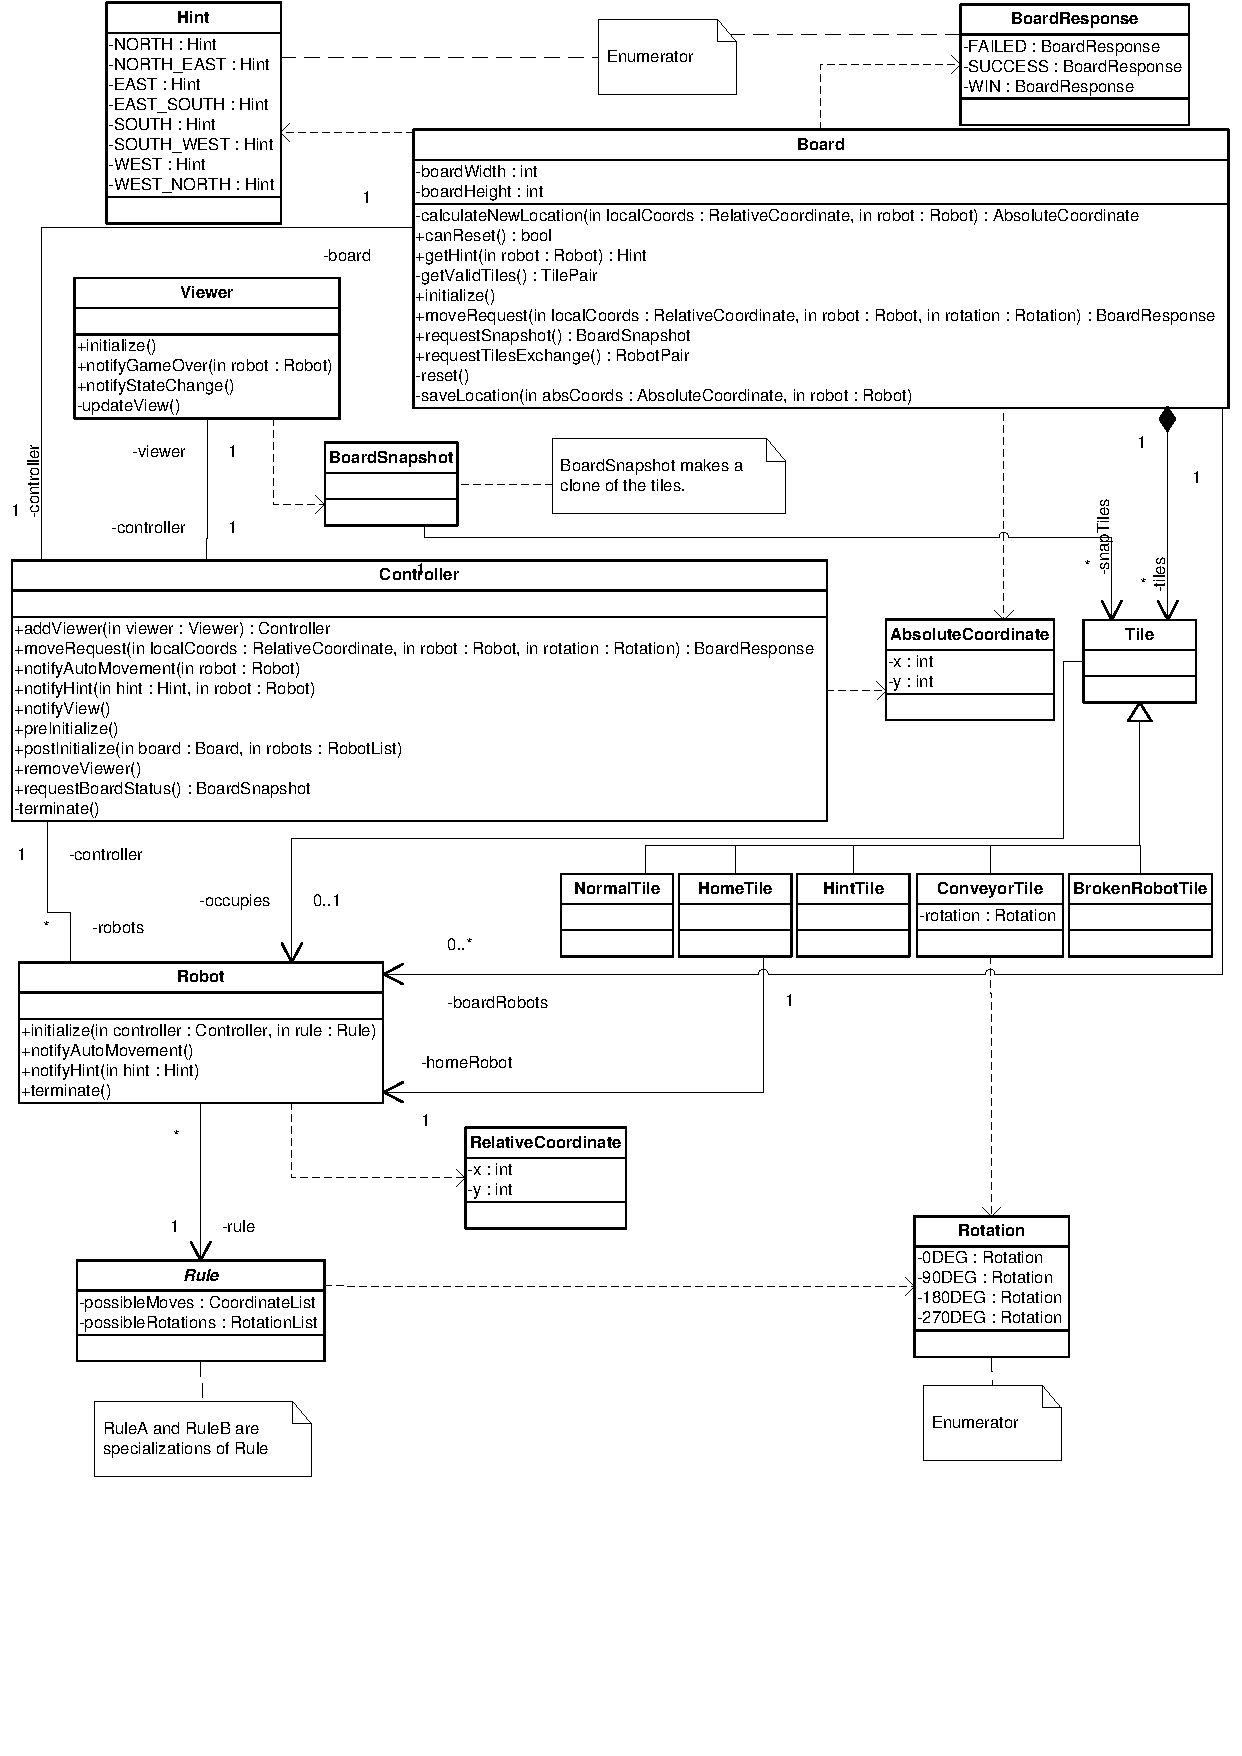
\includegraphics[width=\linewidth]{classdiagram.pdf}
	\let\l=\relax
\let\<=\relax
\let\>=\relax
\digraph[scale=.5]{classdiagram}{
margin=0
fontsize=8
fontname=Helvetica
compound=true
splines=ortho
node [fontsize=8, fontname=Helvetica, shape=record]
edge [fontsize=8, fontname=Helvetica, arrowhead=open, labeldistance=2]
Board [label="{Board|- width : int\l- height : int\l|+ canReset() : bool\l+ initialize()\l+ moveRequest(loc : RelativeCoord, r : Robot, rot : Rotation) : BoardResponse\l+ requestSnapshot() : BoardSnapshot\l+ requestTilesExchange() : bool\l- getHint(r : Robot) : Hint\l- calculateNewLocation(loc : RelativeCoord, r : Robot) :
AbsoluteCoord\l- getValidTiles() : TilePair\l- reset()\l- saveLocation(loc : AbsoluteCoord, r : Robot)\l}"]
Hint [label="{[Hint]| NORTH\l NORTH_EAST\l EAST\l SOUTH_EAST\l SOUTH\l SOUTH_WEST\l WEST\l NORTH_WEST\l}"]
BoardResponse [label="{[BoardResponse]| FAILED\l SUCCESS\l WIN\l}"]
Viewer [label="{Viewer||+ initialize()\l+ notifyGameOver(r : Robot)\l+ notifyStateChange()\l- updateView()\l}"]
BoardSnapshot [label="{BoardSnapshot||}"]
Controller [label="{Controller||+ addViewer(v : Viewer) : Controller\l+ moveRequest(loc : RelativeCoord, r : Robot, rot : Rotation) : BoardResponse\l+ notifyAutoMovement(r : Robot)\l+ notifyHint(h : Hint, r : Robot)\l+ notifyView()\l+ preInitialize()\l+ postInitialize(b : Board, rs : RobotList)\l+ removeViewer()\l+ requestBoardSnapshot() : BoardSnapshot\l- terminate()\l}"]
AbsoluteCoord [label="{AbsoluteCoord|+ x : int\l+ y : int\l|}"]
Tile [label="{Tile||}"]
/**/
subgraph cluster_Tiles {
NormalTile [label="{NormalTile||}"]
HomeTile [label="{HomeTile||}"]
HintTile [label="{HintTile||}"]
ConveyorTile [label="{ConveyorTile|- rot : Rotation|}"]
BrokenRobotTile [label="{BrokenRobotTile||}"]
}
/**/
Robot [label="{Robot||+ initialize(c : Controller, r : Rule)\l+ notifyAutoMovement()\l+ notifyHint(h : Hint)\l+ terminate()\l}"]
RelativeCoord [label="{RelativeCoord|+ x : int\l+ y : int\l|}"]
Rule [label="{\<\<Rule\>\>|- possibleMoves : RelativeCoordList\l- possibleRotations : RotataionList\l|}"]
Rotation [label="{[Rotation]| 0DEG\l 90DEG\l 180DEG\l 270DEG\l}"]
/**/
Board->Controller [taillabel=1, headlabel="0..*"]
Board->Tile [arrowtail=diamond,dir=both, taillabel=1,headlabel="*"]
Board->Robot [taillabel=1, headlabel="0..*"]
/**/
Controller->Viewer [taillabel=1, headlabel=1, arrowhead=none]
Controller->Robot [taillabel=1, headlabel="*", arrowhead=none]
/**/
Tile->Robot [taillabel=1, headlabel="              0..1 - occupier"]
/**/
HomeTile->Robot [taillabel=1, headlabel="              1 - homeRobot"]
/**/
Robot->Rule [taillabel="*", headlabel=1]
/**/
BoardSnapshot->Tile [taillabel=1, headlabel="*"]
/**/
NormalTile->Tile [ltail=cluster_Tiles,arrowhead=empty]
/**/
Board->Hint [style=dashed]
Board->BoardResponse [style=dashed]
Board->AbsoluteCoord [style=dashed]
Viewer->BoardSnapshot [style=dashed]
Controller->AbsoluteCoord [style=dashed]
Robot->RelativeCoord [style=dashed]
Rule->Rotation [style=dashed]
ConveyorTile->Rotation [style=dashed]
} 
    Abstract classes are indicated by guillemets and enumerators by brackets.

\subsection{Class description}
    Next, a description will be given about all the classes in the class diagram. Here, the function of the class can be found, along with its attributes and its functions (and description of these). Since some of the functions have a lot of arguments, these arguments are not showed here. Note that most relations in the class diagram are undirected; for example, the robot has no knowledge about the board, so the association between Board and Robot is directed. The controller and the viewer, however, do have knowledge about each other, so this is an undirected association.

	\begin{description}
        \item[Hint] An enumeration that contains all possible hints that a Robot can receive from a hint tile.
        \item[BoardResponse] An enumerator that contains all the possible responses that the board can give the controller when it makes a move request.
		\item[Board] This class contains the functionality of the board. It contains the following attributes:
        \begin{description}
            \item width: The private variable which contains the width of the board.
            \item height: The private variable which contains the height of the board.
        \end{description}
        Furthermore, the following functions are present:
        \begin{description}
            \item canReset(): The public method which checks if the board can reset. The board can reset if a robot has reached its home tile and a new game can begin.
            \item initialize(): The public method to initialize the board (and with this, also the controller and the robots).
            \item moveRequest(): The public method which handles move requests forwarded by the controller. This method first checks if the move is valid (otherwise, return the BoardResponse FAILED), next it calls calculateNewLocation() to calculate the new location of the robot. After that, saveLocation is called to save the location and the proper board response is returned. Sometimes the board also sends a hint or a notification of an automovement.
            \item requestTilesExchange(): This public method handles with the tiles exchange after a robot has made his move. First it calls getValidTiles() to make sure that the invariant still holds after the exchange. Next it swaps the tiles and handles possible robot replacements or movements.
            \item getHint(): This private method gets an appropriate hint for the robot.
            \item calculateNewLocation(): This private method (used in moveRequest()) calculates the new location of a robot, according to his current position and the position he wants to move to. It also deals with conveyor tiles and broken robot tiles.
            \item getValidTiles(): This private method is used to get two tiles that can be switched, hereby not violating the invariant.
            \item reset(): This private method is used to reset the board. canReset() should return true in order for this function to be called. The board then makes the other components terminate and can initiate new components (e.g. controller, robots) in order to start a new game.
            \item saveLocation(): This private method is used to save the new location of a robot; it is called in moveRequest().
        \end{description}
		\item[Controller] This class represents the controller, which is used as mostly used as communication device between the board and other components. The controller has a viewer, as shown on the undirected association between Controller and Viewer. The controller has the following functions:
        \begin{description}
            \item addViewer(): This public method is used to add a viewer to the controller, so that the controller can notify this viewer when there is a change in the board (see the association in the class diagram).
            \item moveRequest(): This public method is used to forward move requests from the robot. The robot calls this function and the controller calls the moveRequest() function from the board with the right parameters.
            \item notifyAutoMovement(): This public method is used to notify the robot that is has been moved without the robot wanting to; for example, because of a conveyor tile or a tiles exchange.
            \item notifyHint(): This public method is used to notify a robot that it is on a hint tile and what direction he has to go in order to find his home tile.
            \item notifyViewer(): This public method is used to notify the viewer that the board has changed. A snapshot will be send to the viewer.
            \item preInitialize(): This public method is used to pre-initialize the controller, so that there exists an object of the type controller.
            \item postInitialize(): This public method is used to (after pre-initialization) fully initialize the controller with a board and the robots.
            \item removeViewer(): This public method is used to remove a viewer from the controller. This function can be used to add a new viewer or before termination.
            \item terminate(): This function is used to first terminate all objects (except for board). After these objects have been terminated, it informs the board about this; afterwards, the controller itself terminates.
        \end{description}
        \item[Viewer] This class describes the functionality of the viewer, so that the game can be watched. This class has no special attributes. It contains the following functions:
        \begin{description}
            \item initialize(): This public method is used to initialize a viewer.
            \item notifyGameOver(): This public method is used to notify the viewer that a robot has reached its home tile. Fireworks will be shown and after this the viewer can terminate.
            \item notifyStateChange(): This public method is used to notify the viewer that the board has changed, hereby receiving a new snapshot of the board. After this, updateView() will be called to deal with the new snapshot.
            \item updateView(): This private method deals with new snapshots of the board and makes sure that they will be shown.
        \end{description}
        \item[AbsoluteCoord] A data class that contains the x and y coordinate of an absolute coordinate.
		\item[BoardSnapshot] A data class that contains a snapshot of the board, i.e. a copy of all the tiles in the board.
		\item[Tile] Used to model the tiles that the Board consists of.
		\item[NormalTile] Tiles without a special meaning (specialization of the Tile class).
		\item[HomeTile] Tiles that are the "home" of a robot (specialization of the Tile class).
		\item[HintTile] Tiles that return a hint as to where the robot's home is (specialization of the Tile class).
		\item[ConveyorTile] Tiles that change the position and rotation of robots (specialization of the Tile class).
		\item[BrokenRobotTile] Tiles that are occupied by a defective robot (specialization of the Tile class).
		\item[Robot] This class is used for the functionality of robots, both of type A or B in the informal specification. This class has a rule, as shown on the directed association between Robot and Rule. This class has the following functions:
        \begin{description}
            \item initialize(): This public method is used to initialize a given robot, hereby also initializing its rule, a robot of type A or B will then start.
            \item notifyAutomovement(): This public method is used to notify the robot that it has been moved automatically (e.g. by a conveyor tile or by the tiles exchange).
            \item notifyHint(): This public method is used to notify a robot that it has stepped on a hint tile and what direction he has to go in order to find his home tile.
            \item terminate(): This public method is used to make the robot terminate.
        \end{description}
		\item[Rule] An abstract class that is used to model the behaviour of Robot A and B in the Robot class. Any class that defines a rule inherits from this class. This class does not contain any functions. This class has the following attributes:
        \begin{description}
            \item possibleMoves: A list of relative coordinates where the robot is allowed to move to.
            \item possibleRotations: A list of rotations the robot is allowed to do.
        \end{description}
		\item[RelativeCoord] A data class that contains the x and y coordinate of a relative coordinate.
		\item[Rotation] An enumeration that is used to model the rotation in robots and conveyors.
	\end{description}

    ToDo

    \section{Remarks about Message Sequence Chart}
	%\subsection{Class diagram}
	The following graphic is the class diagram that will be used for the specification and the implementation. Note that, for the sake of readability, names of parameters in methods are abbreviated. For instance, the parameter 'loc' in the moveRequest of Board is in the MSCs referred to as 'localCoords', whereas in the class diagram it is abbreviated.

	%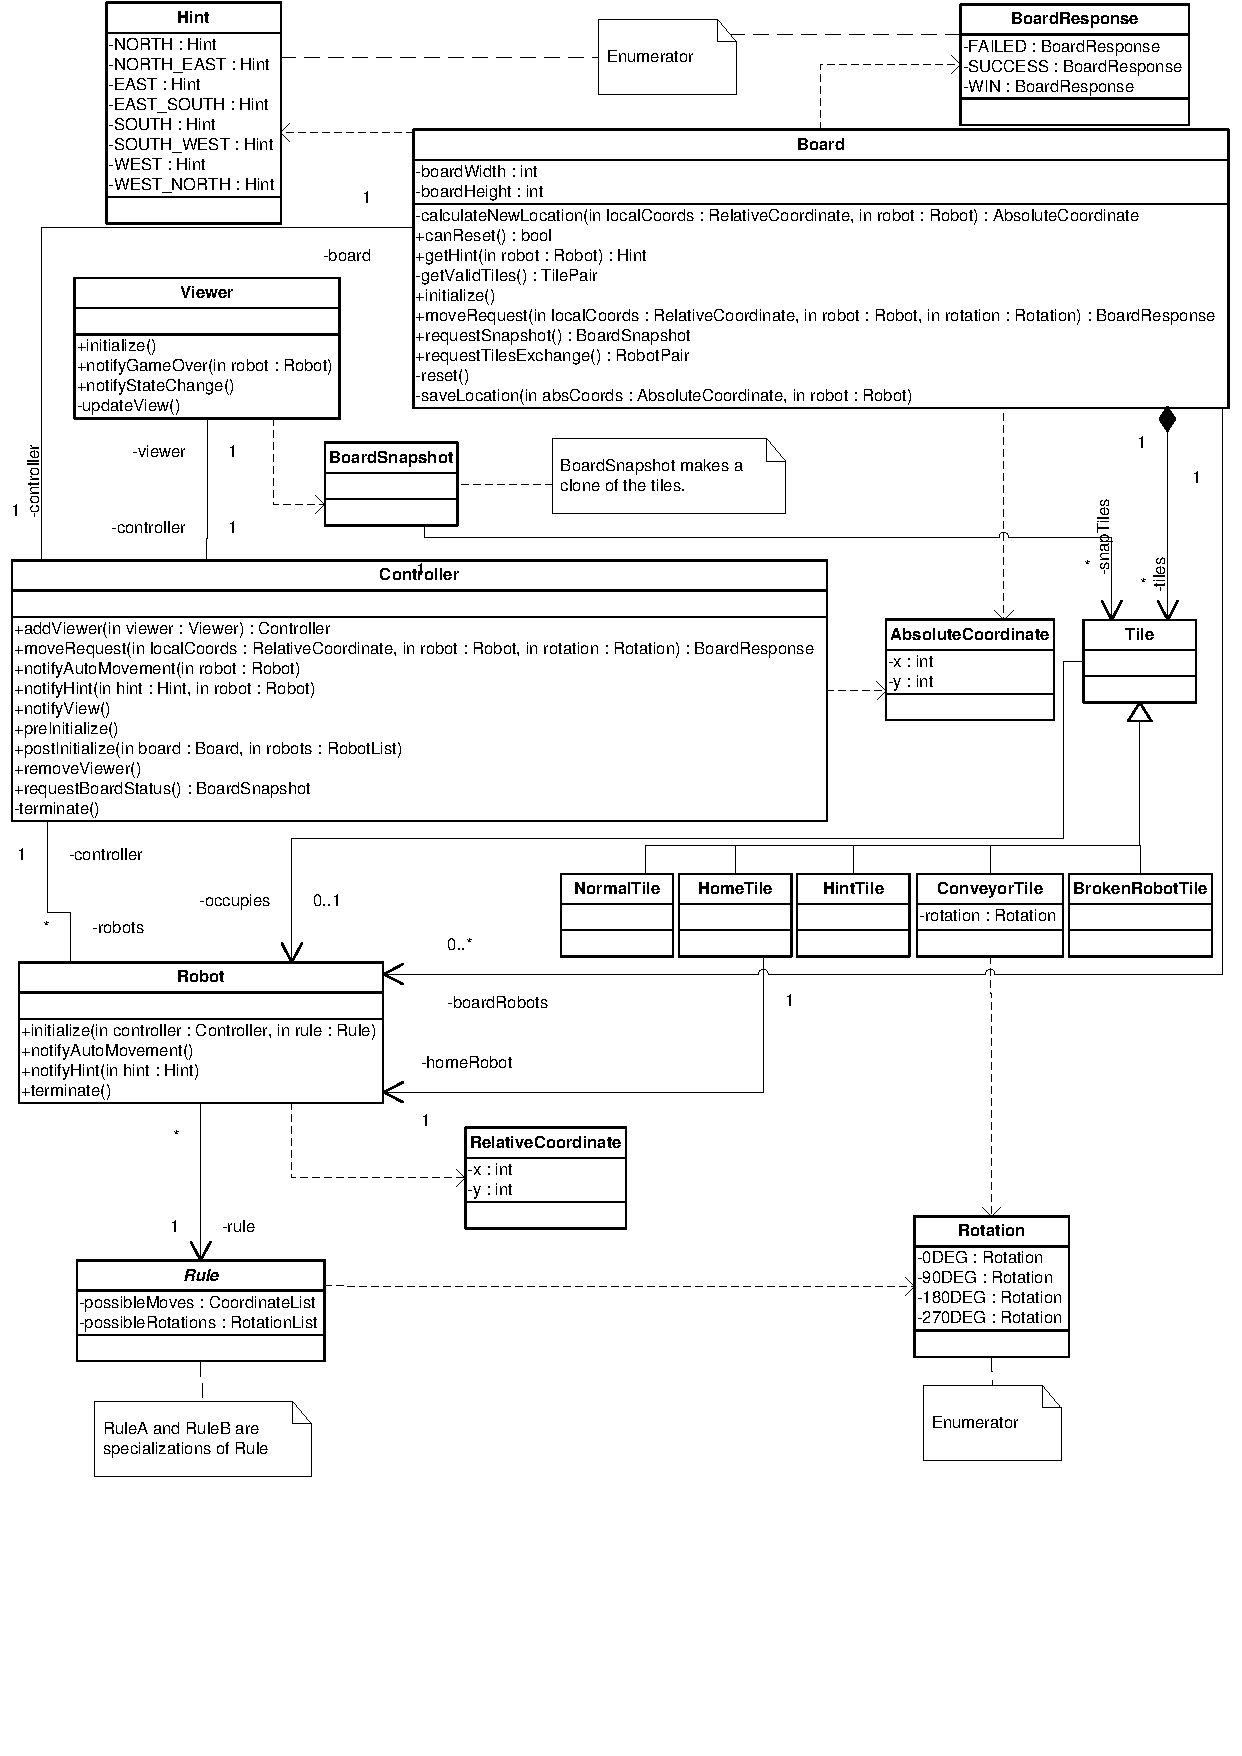
\includegraphics[width=\linewidth]{classdiagram.pdf}
	\let\l=\relax
\let\<=\relax
\let\>=\relax
\digraph[scale=.5]{classdiagram}{
margin=0
fontsize=8
fontname=Helvetica
compound=true
splines=ortho
node [fontsize=8, fontname=Helvetica, shape=record]
edge [fontsize=8, fontname=Helvetica, arrowhead=open, labeldistance=2]
Board [label="{Board|- width : int\l- height : int\l|+ canReset() : bool\l+ initialize()\l+ moveRequest(loc : RelativeCoord, r : Robot, rot : Rotation) : BoardResponse\l+ requestSnapshot() : BoardSnapshot\l+ requestTilesExchange() : bool\l- getHint(r : Robot) : Hint\l- calculateNewLocation(loc : RelativeCoord, r : Robot) :
AbsoluteCoord\l- getValidTiles() : TilePair\l- reset()\l- saveLocation(loc : AbsoluteCoord, r : Robot)\l}"]
Hint [label="{[Hint]| NORTH\l NORTH_EAST\l EAST\l SOUTH_EAST\l SOUTH\l SOUTH_WEST\l WEST\l NORTH_WEST\l}"]
BoardResponse [label="{[BoardResponse]| FAILED\l SUCCESS\l WIN\l}"]
Viewer [label="{Viewer||+ initialize()\l+ notifyGameOver(r : Robot)\l+ notifyStateChange()\l- updateView()\l}"]
BoardSnapshot [label="{BoardSnapshot||}"]
Controller [label="{Controller||+ addViewer(v : Viewer) : Controller\l+ moveRequest(loc : RelativeCoord, r : Robot, rot : Rotation) : BoardResponse\l+ notifyAutoMovement(r : Robot)\l+ notifyHint(h : Hint, r : Robot)\l+ notifyView()\l+ preInitialize()\l+ postInitialize(b : Board, rs : RobotList)\l+ removeViewer()\l+ requestBoardSnapshot() : BoardSnapshot\l- terminate()\l}"]
AbsoluteCoord [label="{AbsoluteCoord|+ x : int\l+ y : int\l|}"]
Tile [label="{Tile||}"]
/**/
subgraph cluster_Tiles {
NormalTile [label="{NormalTile||}"]
HomeTile [label="{HomeTile||}"]
HintTile [label="{HintTile||}"]
ConveyorTile [label="{ConveyorTile|- rot : Rotation|}"]
BrokenRobotTile [label="{BrokenRobotTile||}"]
}
/**/
Robot [label="{Robot||+ initialize(c : Controller, r : Rule)\l+ notifyAutoMovement()\l+ notifyHint(h : Hint)\l+ terminate()\l}"]
RelativeCoord [label="{RelativeCoord|+ x : int\l+ y : int\l|}"]
Rule [label="{\<\<Rule\>\>|- possibleMoves : RelativeCoordList\l- possibleRotations : RotataionList\l|}"]
Rotation [label="{[Rotation]| 0DEG\l 90DEG\l 180DEG\l 270DEG\l}"]
/**/
Board->Controller [taillabel=1, headlabel="0..*"]
Board->Tile [arrowtail=diamond,dir=both, taillabel=1,headlabel="*"]
Board->Robot [taillabel=1, headlabel="0..*"]
/**/
Controller->Viewer [taillabel=1, headlabel=1, arrowhead=none]
Controller->Robot [taillabel=1, headlabel="*", arrowhead=none]
/**/
Tile->Robot [taillabel=1, headlabel="              0..1 - occupier"]
/**/
HomeTile->Robot [taillabel=1, headlabel="              1 - homeRobot"]
/**/
Robot->Rule [taillabel="*", headlabel=1]
/**/
BoardSnapshot->Tile [taillabel=1, headlabel="*"]
/**/
NormalTile->Tile [ltail=cluster_Tiles,arrowhead=empty]
/**/
Board->Hint [style=dashed]
Board->BoardResponse [style=dashed]
Board->AbsoluteCoord [style=dashed]
Viewer->BoardSnapshot [style=dashed]
Controller->AbsoluteCoord [style=dashed]
Robot->RelativeCoord [style=dashed]
Rule->Rotation [style=dashed]
ConveyorTile->Rotation [style=dashed]
} 
    Abstract classes are indicated by guillemets and enumerators by brackets.

\subsection{Class description}
    Next, a description will be given about all the classes in the class diagram. Here, the function of the class can be found, along with its attributes and its functions (and description of these). Since some of the functions have a lot of arguments, these arguments are not showed here. Note that most relations in the class diagram are undirected; for example, the robot has no knowledge about the board, so the association between Board and Robot is directed. The controller and the viewer, however, do have knowledge about each other, so this is an undirected association.

	\begin{description}
        \item[Hint] An enumeration that contains all possible hints that a Robot can receive from a hint tile.
        \item[BoardResponse] An enumerator that contains all the possible responses that the board can give the controller when it makes a move request.
		\item[Board] This class contains the functionality of the board. It contains the following attributes:
        \begin{description}
            \item width: The private variable which contains the width of the board.
            \item height: The private variable which contains the height of the board.
        \end{description}
        Furthermore, the following functions are present:
        \begin{description}
            \item canReset(): The public method which checks if the board can reset. The board can reset if a robot has reached its home tile and a new game can begin.
            \item initialize(): The public method to initialize the board (and with this, also the controller and the robots).
            \item moveRequest(): The public method which handles move requests forwarded by the controller. This method first checks if the move is valid (otherwise, return the BoardResponse FAILED), next it calls calculateNewLocation() to calculate the new location of the robot. After that, saveLocation is called to save the location and the proper board response is returned. Sometimes the board also sends a hint or a notification of an automovement.
            \item requestTilesExchange(): This public method handles with the tiles exchange after a robot has made his move. First it calls getValidTiles() to make sure that the invariant still holds after the exchange. Next it swaps the tiles and handles possible robot replacements or movements.
            \item getHint(): This private method gets an appropriate hint for the robot.
            \item calculateNewLocation(): This private method (used in moveRequest()) calculates the new location of a robot, according to his current position and the position he wants to move to. It also deals with conveyor tiles and broken robot tiles.
            \item getValidTiles(): This private method is used to get two tiles that can be switched, hereby not violating the invariant.
            \item reset(): This private method is used to reset the board. canReset() should return true in order for this function to be called. The board then makes the other components terminate and can initiate new components (e.g. controller, robots) in order to start a new game.
            \item saveLocation(): This private method is used to save the new location of a robot; it is called in moveRequest().
        \end{description}
		\item[Controller] This class represents the controller, which is used as mostly used as communication device between the board and other components. The controller has a viewer, as shown on the undirected association between Controller and Viewer. The controller has the following functions:
        \begin{description}
            \item addViewer(): This public method is used to add a viewer to the controller, so that the controller can notify this viewer when there is a change in the board (see the association in the class diagram).
            \item moveRequest(): This public method is used to forward move requests from the robot. The robot calls this function and the controller calls the moveRequest() function from the board with the right parameters.
            \item notifyAutoMovement(): This public method is used to notify the robot that is has been moved without the robot wanting to; for example, because of a conveyor tile or a tiles exchange.
            \item notifyHint(): This public method is used to notify a robot that it is on a hint tile and what direction he has to go in order to find his home tile.
            \item notifyViewer(): This public method is used to notify the viewer that the board has changed. A snapshot will be send to the viewer.
            \item preInitialize(): This public method is used to pre-initialize the controller, so that there exists an object of the type controller.
            \item postInitialize(): This public method is used to (after pre-initialization) fully initialize the controller with a board and the robots.
            \item removeViewer(): This public method is used to remove a viewer from the controller. This function can be used to add a new viewer or before termination.
            \item terminate(): This function is used to first terminate all objects (except for board). After these objects have been terminated, it informs the board about this; afterwards, the controller itself terminates.
        \end{description}
        \item[Viewer] This class describes the functionality of the viewer, so that the game can be watched. This class has no special attributes. It contains the following functions:
        \begin{description}
            \item initialize(): This public method is used to initialize a viewer.
            \item notifyGameOver(): This public method is used to notify the viewer that a robot has reached its home tile. Fireworks will be shown and after this the viewer can terminate.
            \item notifyStateChange(): This public method is used to notify the viewer that the board has changed, hereby receiving a new snapshot of the board. After this, updateView() will be called to deal with the new snapshot.
            \item updateView(): This private method deals with new snapshots of the board and makes sure that they will be shown.
        \end{description}
        \item[AbsoluteCoord] A data class that contains the x and y coordinate of an absolute coordinate.
		\item[BoardSnapshot] A data class that contains a snapshot of the board, i.e. a copy of all the tiles in the board.
		\item[Tile] Used to model the tiles that the Board consists of.
		\item[NormalTile] Tiles without a special meaning (specialization of the Tile class).
		\item[HomeTile] Tiles that are the "home" of a robot (specialization of the Tile class).
		\item[HintTile] Tiles that return a hint as to where the robot's home is (specialization of the Tile class).
		\item[ConveyorTile] Tiles that change the position and rotation of robots (specialization of the Tile class).
		\item[BrokenRobotTile] Tiles that are occupied by a defective robot (specialization of the Tile class).
		\item[Robot] This class is used for the functionality of robots, both of type A or B in the informal specification. This class has a rule, as shown on the directed association between Robot and Rule. This class has the following functions:
        \begin{description}
            \item initialize(): This public method is used to initialize a given robot, hereby also initializing its rule, a robot of type A or B will then start.
            \item notifyAutomovement(): This public method is used to notify the robot that it has been moved automatically (e.g. by a conveyor tile or by the tiles exchange).
            \item notifyHint(): This public method is used to notify a robot that it has stepped on a hint tile and what direction he has to go in order to find his home tile.
            \item terminate(): This public method is used to make the robot terminate.
        \end{description}
		\item[Rule] An abstract class that is used to model the behaviour of Robot A and B in the Robot class. Any class that defines a rule inherits from this class. This class does not contain any functions. This class has the following attributes:
        \begin{description}
            \item possibleMoves: A list of relative coordinates where the robot is allowed to move to.
            \item possibleRotations: A list of rotations the robot is allowed to do.
        \end{description}
		\item[RelativeCoord] A data class that contains the x and y coordinate of a relative coordinate.
		\item[Rotation] An enumeration that is used to model the rotation in robots and conveyors.
	\end{description}

    ToDo
    
    \section{Judgement and grading}
    ToDo

\end{document} 